%!TEX root = ../physical-olympics-2.tex
\chapter{静力学}

以运动学和动力学理论为基础,\,时不时地,\,我们发现一些典型的现象,\,包括:
\begin{itemize}
	\item 不管体系多么复杂,\,能量函数对其行为似乎起决定性的作用.
	\item 似乎总是能够从不同的体系中抽象出它的一个特征数字:\,自由度.
	\item 约束越多体系约复杂,\,它的未知约束力越来越多,\,但是多到一定程度体系只剩下一个自由度了反而用能量守恒就能够解答大多数问题.
\end{itemize}

这些现象无疑是紧密联系的,\,值得研究的.\,事实上我们要做的就是以之前的所有动力学定律为依据进一步展开讨论.\,再从头开始建立新的理论:\,先讨论运动的描述,\,再单独研究力的特性.\,最后合到一起,\,看看这能让我们得到什么.

新理论,\, 新思想,\, 新图像.\,在本章节的学习过程中,\, 如果感到疑惑,\, 大抵都是复杂的数学推导掩盖了背后的物理目的.\, 希望读者先记住两点:\,一是,\,我们要做的是把以前对质点,\,刚体和对质点系列的选取自然坐标(大抵是直角座标)而列的部分定理修改为改用广义坐标来描述,\,过程中的所有步骤都是为这个目的来服务的.\, 二是,\,本着``能量函数的形式''就决定``体系的一切结构与演化''的观点,\,我们就能找到一个明确的方向.\,无论是从结果上还是从细节上,\,我们将会多次参考这种想法.

\section{约束}
所谓\emph{约束}(constraint)就是对运动的限制.\,有时,\,物体发生直接的接触,\,或是一个物体在另一个物体表面滑动或是滚动,\,这种情况约束实际上就发生了;\,有时,\,约束通过往往是轻质\footnote{后面就能理解,\,这样才不会占用新的广义坐标,\,因为它不带来任何能量}的绳,\,直杆或曲杆,\,套筒,\,无摩擦的铰链等等去连接两个乃至多个物体,\,这样那些物体之间实际上也存在约束,\,偶尔我们也会把连接它们的机构直接叫做约束.

之所以把它们叫做约束,\,是因为它们产生了两个共同的结果,\,一是约束方程,\,二是约束力.\,根据前者的运动学效果\footnote{根据后者的动力学效果还可以分为理想和非理想约束,\,见后面小节平衡问题:\,虚功原理},\,我们把与约束分为以下类别:

\subsection{约束分类}

无论是挂在天花板下的小球,\,还是``鹰击长空,\,鱼翔浅底'',\,都给我们以\emph{单边约束}(unilateral constraint)的图像.
\begin{figure}[H]
\centering
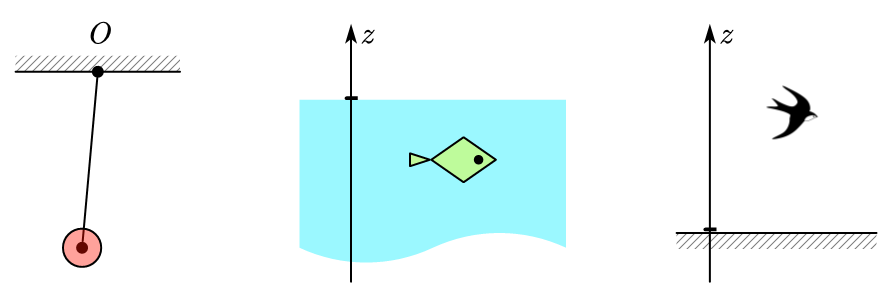
\includegraphics[width=14cm]{image/6-2-1.png}
\caption{可解约束}
\end{figure}

更简单的例子还包括两个物体表面发生接触(滑动或滚动)的情况.\,此时,\,

\subsection{广义坐标与自由度}

\subsection{约束力与广义力}

\subsection{完整约束}

\section{力系化简}

\subsection{公理化静力学体系}

\subsection{力系向一点简化}

\section{平衡问题:\,矢量力学}

\subsection{平衡问题的要素}

\subsection{平衡条件与判据}

\subsection{负静定,\,静定与超静定}

\subsection{静摩擦的临界}

\section{平衡问题:\,虚功原理}

\subsection{理想约束}

\subsection{负静定问题的虚功原理}

\subsection{静定,\,超静定问题的求解}

\section{分析力学初步*}

\subsection{用广义坐标表示能量}

\subsection{拉格朗日方程}

\subsection{再论冲击问题}

\subsection{哈密顿力学简介}

\section{平衡态稳定性}

\subsection{一自由度体系}

\subsection{多自由度体系}
